\usepackage{graphicx}
\newpage
\thispagestyle{fancy}
\vspace{\fill}

\subsection{Ajuste de pressão no Porta Manta}
\begin{figure}
    \centering
    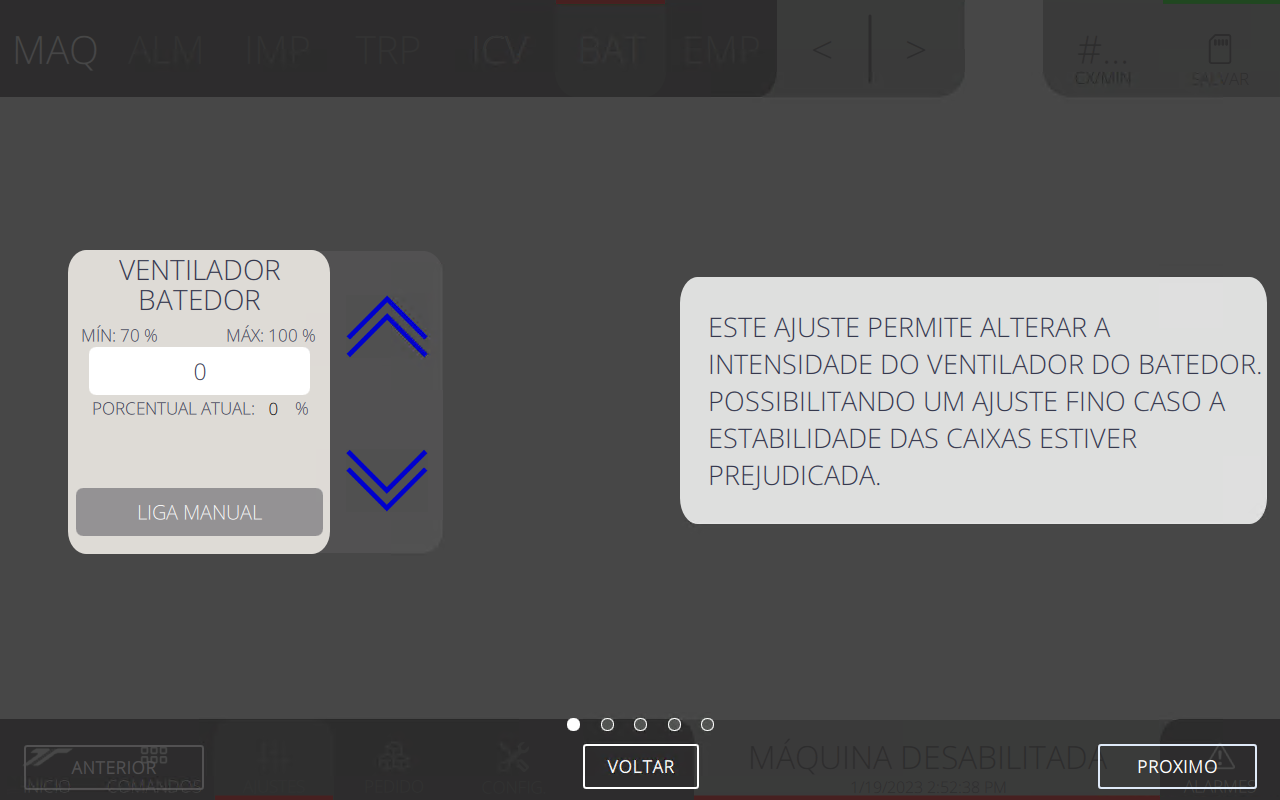
\includegraphics[width=480,height=300]{imagesICV/06-dryCutter/commands/e-1}
    \caption{Ajuste de pressão no Porta Manta}
\end{figure}
\newpage
\thispagestyle{fancy}
\vspace{\fill}

\subsection{Executa ponto zero}
\begin{figure}
    \centering
    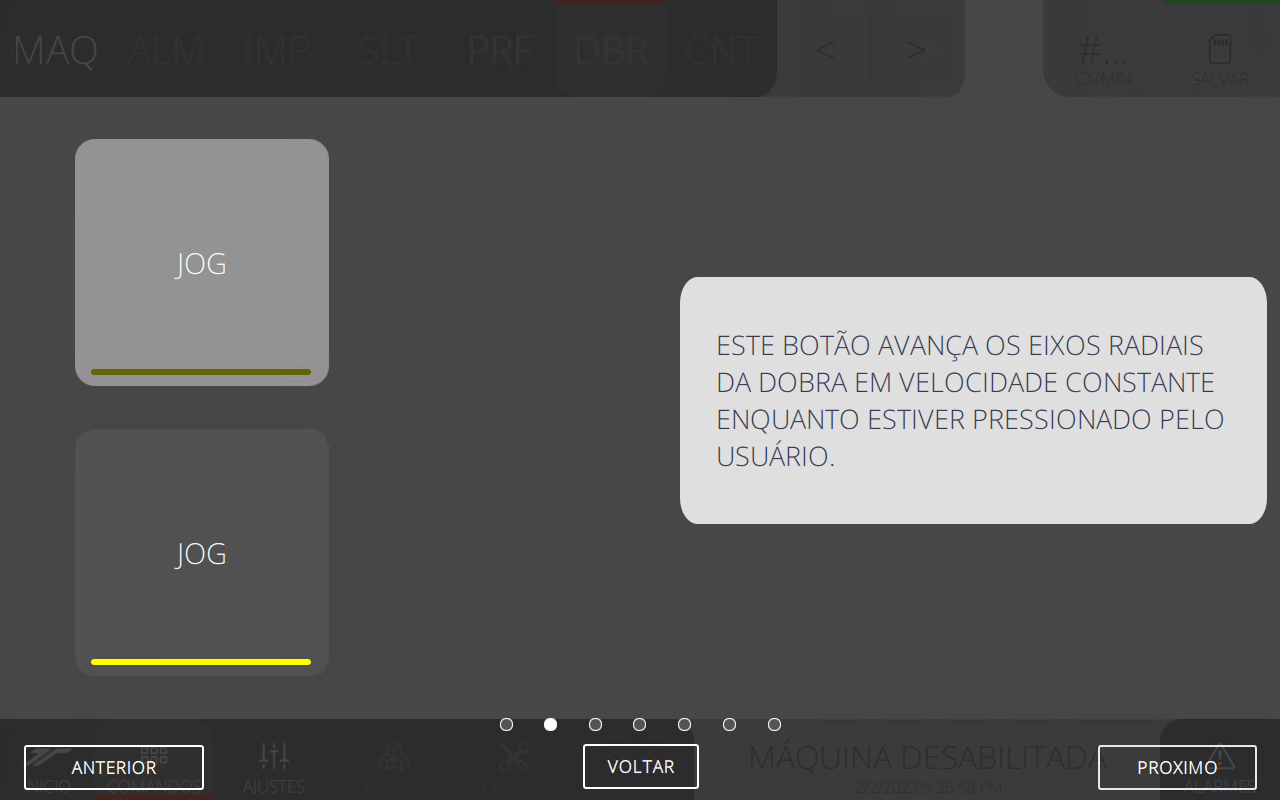
\includegraphics[width=576,height=360]{imagesICV/06-dryCutter/commands/e-2}
    \caption{Executa ponto zero}
\end{figure}
\newpage
\thispagestyle{fancy}
\vspace{\fill}

\subsection{Trava unidade Corte e Vinco na unidade Batedor}
\begin{figure}
    \centering
    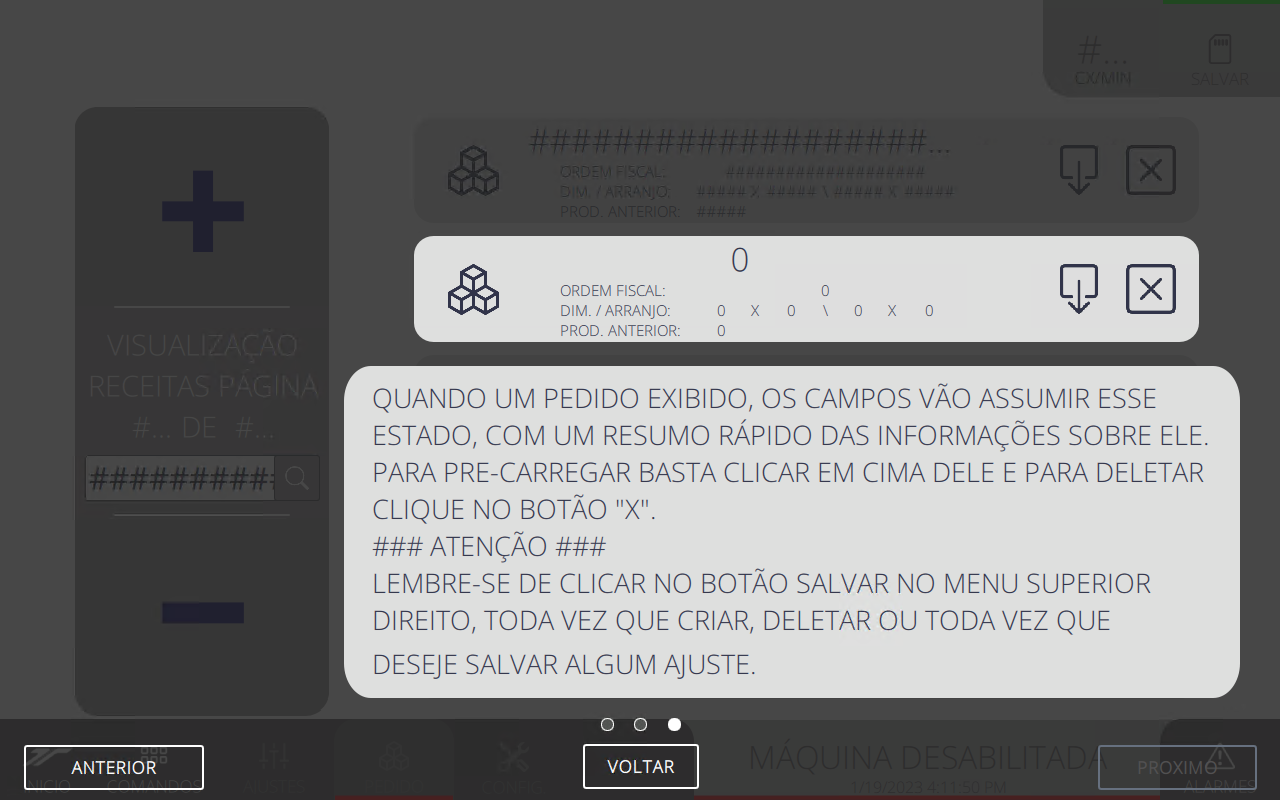
\includegraphics[width=576,height=360]{imagesICV/06-dryCutter/commands/e-3}
    \caption{Trava unidade Corte e Vinco na unidade Batedor}
\end{figure}
\newpage
\thispagestyle{fancy}
\vspace{\fill}

\subsection{Habilita transporte de refiles}
\begin{figure}
    \centering
    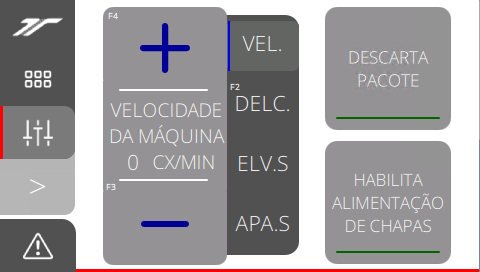
\includegraphics[width=576,height=360]{imagesICV/06-dryCutter/commands/e-4}
    \caption{Habilita transporte de refiles}
\end{figure}
\newpage
\thispagestyle{fancy}
\vspace{\fill}